
\documentclass{article}
\usepackage{graphicx} % Required for inserting images
\usepackage{fancyhdr} % Required for header and footer configuration
\usepackage[a4paper, margin=2.5cm, left=1.5cm, right=1.5cm, bottom=4cm]{geometry} % Required for setting page margins
\usepackage[T1]{fontenc}
\usepackage[default,oldstyle,scale=1]{opensans} % Utilizzo del font Open Sans
\usepackage{lipsum}
\usepackage{makeidx}
\usepackage{booktabs}
\usepackage{tabularray}
\usepackage[colorlinks=true, linkcolor=black, urlcolor=blue, citecolor=blue]{hyperref}
\usepackage{tabularx}
\usepackage{makecell}
\usepackage{enumitem} % Pacchetto per la personalizzazione degli elenchi
\usepackage{booktabs}
\usepackage{subcaption}

% Configure header and footer for the first page
\fancypagestyle{firstpage}{
    \fancyhf{} % Clear header and footer
    \renewcommand{\headrulewidth}{0pt} % Remove header rule line
    \lhead{} % Header on the left
    \chead{} % Header in the center
    \rhead{} % Header on the right
    \lfoot{} % Footer on the left
    \cfoot{\vspace{5pt}\\\hrulefill\\\vspace{10pt}\textbf{BeeLive}\\Gruppo 21} % Footer in the center
    \rfoot{\vspace{32.5pt}\\\thepage} % Footer on the right
}

% Configure header and footer for non-plain pages (second page onwards)
\fancypagestyle{nonplain}{
    \fancyhf{} % Clear header and footer
    \lhead{} % Header on the left
    \chead{} % Header in the center
    \rhead{
\includegraphics[width=2cm]{Images/BeeLive-Logo.png}\\\vspace{2pt}} % Header on the right
    \lfoot{} % Footer on the left
    \cfoot{\vspace{5pt}\\\hrulefill\\\vspace{10pt}\textbf{BeeLive}\\Gruppo 21} % Footer in the center
    \rfoot{\vspace{32.5pt}\\\thepage} % Footer on the right
}

% Adjust vertical space between header and text                                    
\setlength{\headsep}{65pt} 
% Adjust vertical space between text and footer
\setlength{\footskip}{0pt} 

\title{
\includegraphics[width=0.75\textwidth]{Images/BeeLive-Logo.png}\\\vspace{100pt}
\LARGE{\textbf{BeeLive\\Deliverable 2}}}
\author{Gruppo 21:\\
Cipriani Pietro, 226959\\
Orlando Dennis, 227688\\
Ziviani Elia, 228172}
\date{22 Aprile 2024}

\makeindex % Indica che vogliamo creare un indice

\begin{document}

\maketitle
\thispagestyle{firstpage} % Apply firstpage style to the first page
\clearpage

\pagestyle{nonplain} % Apply non-plain style to subsequent pages

\renewcommand{\contentsname}{Indice}
\tableofcontents

\clearpage

\section{Component Diagram}
\index{Component Diagram}

Questo capitolo è incentrato sull'analisi dei componenti del sistema che saranno realizzati.\\
Lo scopo è quello di descrivere ogni singolo componente in termini di funzionalità e interfacce.\\

I componenti sono individuati seguendo quando espresso nel documento Deliverable 1 per quanto riguarda i casi d'uso e sono definiti come entità autonome nel sistema.\\
Questi componenti sono provvisti di interfacce che permettono la comunicazione tra di essi.\\
Le interfacce sono definite come:
\begin{itemize}
    \item \textbf{Interfaccia RICHIESTA}: Tutte quelle interfacce che offrono servizi alla componente.
    \item \textbf{Interfaccia FORNITA}: Tutti quelle interfacce che consentono di usufruire dei servizi offerti dalla componente.
\end{itemize} 

\subsection{Diagramma dei componenti overview}
\index{Diagramma dei componenti overview}

\begin{figure}[htbp]
    \centering
    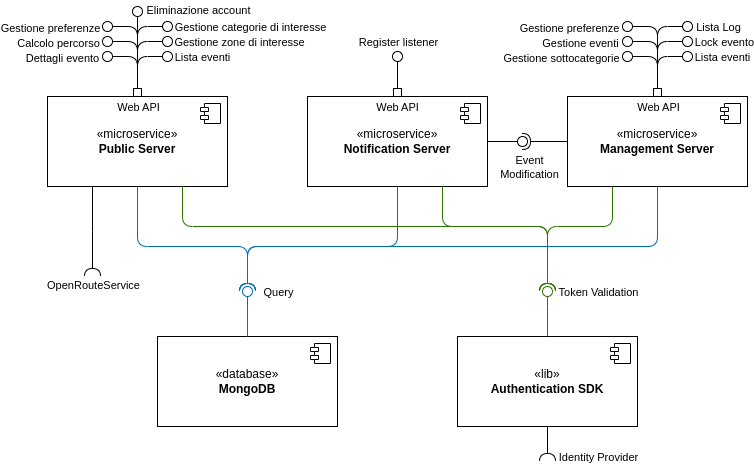
\includegraphics[width=1\textwidth]{Images/ComponentDiagram_overview.png}
    \caption{Diagramma dei componenti overview}
    \label{fig:component-diagram-overview}
\end{figure}

\clearpage

\subsubsection{Public server}
\index{Public server}

\begin{table}[htbp]
    \centering
    \renewcommand{\arraystretch}{1.3} % Imposta lo spazio verticale delle righe
    \begin{tabularx}{\textwidth}{| l | l | X |}
        \Xhline{2pt}
        \textbf{RICHIESTA} & \textbf{Nome} & \textbf{Descrizione} \\
        \Xhline{2pt}
         & OpenRouteService & Il componente utilizza l'interfaccia fornita da un componente esterno per il calcolo dei percorsi di interesse a partire da una lista di waypoints. \\
        \hline
         & Query & Il componente utilizza l'interfaccia fornita dal componente \textit{MongoDB} per eseguire le queries. \\
        \hline
         & Token validation & Il componente utilizza l'interfaccia fornita dal componente \textit{Authentication SDK} per la verifica e validazione del token di autenticazione. \\
        \Xhline{2pt}
        \textbf{FORNITA} & \textbf{Nome} & \textbf{Descrizione} \\
        \Xhline{2pt}
         & Eliminazione account & Il componente fornisce un'interfaccia per permettere l'eliminazione dell'account utente. Comporta la cancellazione dei dati associati all'utente, nelle tempistiche imposte dalla legge. \\
        \hline
         & Gestione categorie & Il componente fornisce un'interfaccia per permettere la gestione delle categorie d'interesse impostate dall'utente. \\
        \hline
        & Gestione zone & Il componente fornisce un'interfaccia per permettere la gestione delle zone d'interesse impostate dall'utente. \\
        \hline
        & Lista eventi & Il componente fornisce un'interfaccia per permettere di ottenere la lista di tutti gli eventi di interesse. \\
        \hline
        & Gestione preferenze & Il componente fornisce un'interfaccia per permettere la gestione delle preferenze dell'utente. \\
        \hline
        & Calcolo percorso & Il componente fornisce un'interfaccia per permettere il calcolo di un percorso d'interesse a partire da una lista di waypoints, consente di astrarre il servizio utilizzato. \\
        \hline
        & Dettagli evento & Il componente fornisce un'interfaccia per permettere la visualizzazione di tutti i dettagli di un singolo evento. \\
        \hline
    \end{tabularx}
    \caption{Tabella Public server}
\end{table}

\subsubsection{Authentication SDK}
\index{Authentication SDK}

\begin{table}[htbp]
    \centering
    \renewcommand{\arraystretch}{1.3} % Imposta lo spazio verticale delle righe
    \begin{tabularx}{\textwidth}{| l | l | X |}
        \Xhline{2pt}
        \textbf{RICHIESTA} & \textbf{Nome} & \textbf{Descrizione} \\
        \Xhline{2pt}
         & Identity provider & Il componente utilizza un'interfaccia esterna per eseguire la connessione e accedere ai servizi offerti dall'Identity provider. \\
        \Xhline{2pt}
        \textbf{FORNITA} & \textbf{Nome} & \textbf{Descrizione} \\
        \Xhline{2pt}
         & Token validation & Il componente fornisce l'interfaccia che si occupa della verifica e validazione del token di autenticazione. \\
        \hline
    \end{tabularx}
    \caption{Tabella Autherntication SDK}
\end{table}

\clearpage

\subsubsection{Management Server}
\index{Management Server}

\begin{table}[htbp]
    \centering
    \renewcommand{\arraystretch}{1.3} % Imposta lo spazio verticale delle righe
    \begin{tabularx}{\textwidth}{| l | l | X |}
        \Xhline{2pt}
        \textbf{RICHIESTA} & \textbf{Nome} & \textbf{Descrizione} \\
        \Xhline{2pt}
         & Event modification & Il componente utilizza l'interfaccia fornita dal componente \textit{Notification Server} per avvisarlo di modifiche agli eventi. \\
        \hline
         & Query & Il componente utilizza l'interfaccia fornita dal componente \textit{MongoDB} per effettuare delle query per svolgere i suoi ruoli. \\
        \hline
         & Token validation & Il componente utilizza l'interfaccia fornita dal componente \textit{Authentication SDK} per la verifica e validazione del token di autenticazione. \\
        \Xhline{2pt}
        \textbf{FORNITA} & \textbf{Nome} & \textbf{Descrizione} \\
        \Xhline{2pt}
         & Gestione preferenze & Il componente fornisce un'interfaccia per permettere la gestione delle preferenze impostabili dall'utente. \\
        \hline
         & Lista LOG & Il componente fornisce un'interfaccia per permettere la visualizzazione dello storico delle modifiche avvenute nel sistema. \\
        \hline
        & Lock evento & Il componente fornisce un'interfaccia per permettere la mutua esclusione ad un evento, per non permetterne l'accesso contemporaneo in caso di eventuali modifiche. \\
        \hline
        & Lista eventi & Il componente fornisce un'interfaccia per visualizzare la lista degli eventi di competenza dell'utente. \\
        \hline
        & Gestione eventi & Il componente fornisce un'interfaccia per gestire gli eventi a sistema, permettendo creazione, modifica ed eliminazione degli eventi di competenza. \\
        \hline
        & Gestione categorie & Il componente fornisce un'interfaccia per gestire tutte le sottocategorie, permettendo la loro creazione, modifica ed eliminazione. \\
        \hline
    \end{tabularx}
    \caption{Tabella Management server}
\end{table}

\subsubsection{MongoDB}
\index{MongoDB}

\begin{table}[htbp]
    \centering
    \renewcommand{\arraystretch}{1.3} % Imposta lo spazio verticale delle righe
    \begin{tabularx}{\textwidth}{| l | l | X |}
        \Xhline{2pt}
        \textbf{FORNITA} & \textbf{Nome} & \textbf{Descrizione} \\
        \Xhline{2pt}
         & Query & Il componente fornisce un'interfaccia per eseguire queries sul database. \\
        \hline
    \end{tabularx}
    \caption{Tabella MongoDB}
\end{table}

\clearpage

\subsubsection{Notification Server}
\index{Notification Server}

\begin{table}[htbp]
    \centering
    \renewcommand{\arraystretch}{1.3} % Imposta lo spazio verticale delle righe
    \begin{tabularx}{\textwidth}{| l | l | X |}
        \Xhline{2pt}
        \textbf{RICHIESTA} & \textbf{Nome} & \textbf{Descrizione} \\
        \Xhline{2pt}
         & Query & Il componente utilizza l'interfaccia fornita dal componente \textit{MongoDB} l'esecuzione delle query. \\
        \hline
         & Token validation & Il componente utilizza l'interfaccia fornita dal componente \textit{Authentication SDK} per la verifica e validazione del token di autenticazione. \\
        \Xhline{2pt}
        \textbf{FORNITA} & \textbf{Nome} & \textbf{Descrizione} \\
        \Xhline{2pt}
         & Register listener & Il componente fornisce un'interfaccia per aprire un canale sulla quale inviare le notifiche. \\
        \hline
         & Event modification & Il componente fornisce un'interfaccia per essere avvisato di modifiche agli eventi. Modifiche che verranno successivamente inoltrate sui listener interessati alla categoria di evento. \\
        \hline
    \end{tabularx}
    \caption{Tabella Notification Server}
\end{table}

\clearpage

\subsection{Diagramma dei componenti di \textit{Notification Server}}
\index{Diagramma dei componenti di notifica}

\begin{figure}[htbp]
    \centering
    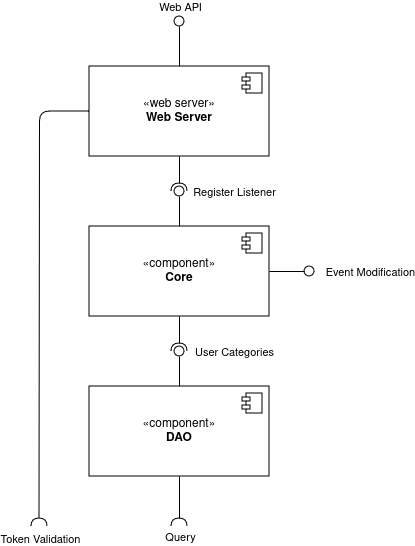
\includegraphics[width=0.5\textwidth]{Images/ComponentDiagram_Notification.drawio.png}
    \caption{Diagramma dei componenti di \textit{Notification Server}}
    \label{fig:component-diagram-notification}
\end{figure}

\subsubsection{DAO}
\index{DAO}

\begin{table}[htbp]
    \centering
    \renewcommand{\arraystretch}{1.3} % Imposta lo spazio verticale delle righe
    \begin{tabularx}{\textwidth}{| l | l | X |}
        \Xhline{2pt}
        \textbf{RICHIESTA} & \textbf{Nome} & \textbf{Descrizione} \\
        \Xhline{2pt}
         & Query & Il componente utilizza un'interfaccia esterna per ottenere tutte le query da eseguire sul database. \\
        \Xhline{2pt}
        \textbf{FORNITA} & \textbf{Nome} & \textbf{Descrizione} \\
        \Xhline{2pt}
         & User categories & Il componente fornisce un'interfaccia per permettere di ottenere tutte le categorie impostate dagli utenti. \\
        \hline
    \end{tabularx}
    \caption{Tabella DAO}
\end{table}

\clearpage

\subsubsection{Web Server}
\index{Web Server}

\begin{table}[htbp]
    \centering
    \renewcommand{\arraystretch}{1.3} % Imposta lo spazio verticale delle righe
    \begin{tabularx}{\textwidth}{| l | l | X |}
        \Xhline{2pt}
        \textbf{RICHIESTA} & \textbf{Nome} & \textbf{Descrizione} \\
        \Xhline{2pt}
         & Token validation & Il componente utilizza l'interfaccia fornita dal componente \textit{Authentication SDK} per la verifica e validazione del token di autenticazione. \\
        \hline
         & Register listener & Il componente utilizza l'interfaccia fornita dal componente \textit{Core} per ricevere le notifiche relative agli eventi. \\
        \Xhline{2pt}
        \textbf{FORNITA} & \textbf{Nome} & \textbf{Descrizione} \\
        \Xhline{2pt}
         & Web API & Il componente fornisce un'interfaccia per permettere l'utilizzo delle API agli applicativi coinvolti nel sistema. \\
        \hline
    \end{tabularx}
    \caption{Tabella Web Server}
\end{table}

\subsubsection{Core}
\index{Core}

\begin{table}[htbp]
    \centering
    \renewcommand{\arraystretch}{1.3} % Imposta lo spazio verticale delle righe
    \begin{tabularx}{\textwidth}{| l | l | X |}
        \Xhline{2pt}
        \textbf{RICHIESTA} & \textbf{Nome} & \textbf{Descrizione} \\
        \Xhline{2pt}
         & User categories & Il componente utilizza l'interfaccia fornita dal componente \textit{DAO} per ottenere tutte le categorie impostate dagli utenti. \\
        \Xhline{2pt}
        \textbf{FORNITA} & \textbf{Nome} & \textbf{Descrizione} \\
        \Xhline{2pt}
         & Event modification & Il componente fornisce un'interfaccia per essere notificato di modifiche agli eventi. \\
        \hline
         & Register listener & Il componente fornisce un'interfaccia per aprire un canale sulla quale inviare le notifiche. \\
        \hline
    \end{tabularx}
    \caption{Tabella Core}
\end{table}

\clearpage

\subsection{Diagramma dei componenti di \textit{Public Server}}
\index{Diagramma dei componenti pubblici}

\begin{figure}[htbp]
    \centering
    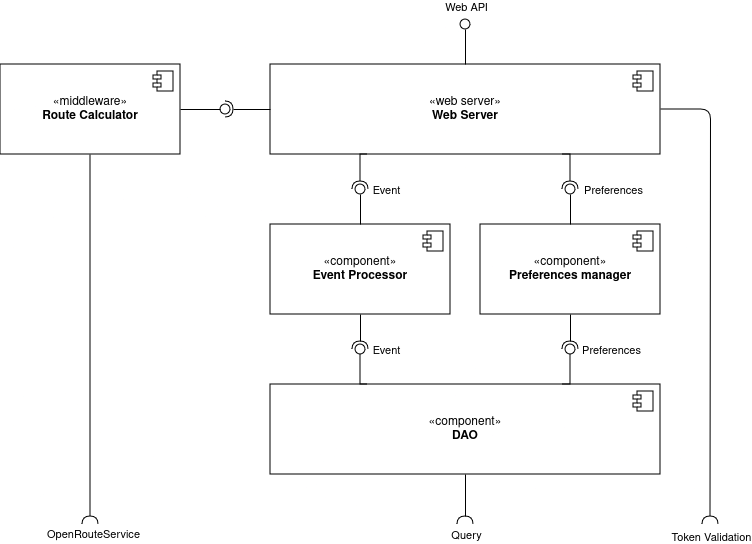
\includegraphics[width=0.75\textwidth]{Images/ComponentDiagram_Public.png}
    \caption{Diagramma dei componenti di \textit{Public Server}}
    \label{fig:component-diagram-public}
\end{figure}

\subsubsection{Route calculator}
\index{Route calculator}

\begin{table}[htbp]
    \centering
    \renewcommand{\arraystretch}{1.3} % Imposta lo spazio verticale delle righe
    \begin{tabularx}{\textwidth}{| l | l | X |}
        \Xhline{2pt}
        \textbf{RICHIESTA} & \textbf{Nome} & \textbf{Descrizione} \\
        \Xhline{2pt}
         & OpenRouteService & Il componente utilizza un'interfaccia esterna per eseguire il calcolo del percorso di interesse dell'utente, a partire da una lista di waypoints. \\
        \Xhline{2pt}
        \textbf{FORNITA} & \textbf{Nome} & \textbf{Descrizione} \\
        \Xhline{2pt}
         & Route & Il componente fornisce un'interfaccia per fornire i percorsi calcolati richiesti dagli utenti. \\
        \hline
    \end{tabularx}
    \caption{Tabella Route calculator}
\end{table}

\clearpage

\subsubsection{Web Server}
\index{Web Server}

\begin{table}[htbp]
    \centering
    \renewcommand{\arraystretch}{1.3} % Imposta lo spazio verticale delle righe
    \begin{tabularx}{\textwidth}{| l | l | X |}
        \Xhline{2pt}
        \textbf{RICHIESTA} & \textbf{Nome} & \textbf{Descrizione} \\
        \Xhline{2pt}
         & Event & Il componente utilizza l'interfaccia fornita dal componente \textit{Event Proessor} per ottenere gli eventi processati dal sistema. \\
        \hline
         & Preferences & Il componente utilizza l'interfaccia fornita dal componente \textit{Preferences manager} per ottenere e modificare le preferenze impostate dagli utenti. \\
        \Xhline{2pt}
        \textbf{FORNITA} & \textbf{Nome} & \textbf{Descrizione} \\
        \Xhline{2pt}
         & Web API & Il componente fornisce un'interfaccia per permettere l'utilizzo delle API agli applicativi coinvolti nel sistema. \\
        \hline
         & Token validation & Il componente utilizza un'interfaccia esterna per eseguire la validazione del token di accesso. \\
        \hline
    \end{tabularx}
    \caption{Tabella Web Server}
\end{table}

\subsubsection{Event processor}
\index{Event processor}

\begin{table}[htbp]
    \centering
    \renewcommand{\arraystretch}{1.3} % Imposta lo spazio verticale delle righe
    \begin{tabularx}{\textwidth}{| l | l | X |}
        \Xhline{2pt}
        \textbf{RICHIESTA} & \textbf{Nome} & \textbf{Descrizione} \\
        \Xhline{2pt}
         & Event & Il componente utilizza l'interfaccia fornita dal componente \textit{DAO} per ottenere gli eventi presenti nel sistema. \\
        \Xhline{2pt}
        \textbf{FORNITA} & \textbf{Nome} & \textbf{Descrizione} \\
        \Xhline{2pt}
         & Event & Il componente fornisce un'interfaccia per fornire gli eventi processati. \\
        \hline
    \end{tabularx}
    \caption{Tabella Event Processor}
\end{table}

\subsubsection{Preferences manager}
\index{Preferences manager}

\begin{table}[htbp]
    \centering
    \renewcommand{\arraystretch}{1.3} % Imposta lo spazio verticale delle righe
    \begin{tabularx}{\textwidth}{| l | l | X |}
        \Xhline{2pt}
        \textbf{RICHIESTA} & \textbf{Nome} & \textbf{Descrizione} \\
        \Xhline{2pt}
         & Preferences & Il componente utilizza l'interfaccia fornita dal componente \textit{DAO} per ottenere e modificare le preferenze impostate dagli utenti. \\
        \Xhline{2pt}
        \textbf{FORNITA} & \textbf{Nome} & \textbf{Descrizione} \\
        \Xhline{2pt}
         & Preferences & Il componente fornisce un'interfaccia per ottenere e modificare le preferenze impostate dagli utenti. \\
        \hline
    \end{tabularx}
    \caption{Tabella Preferences Manager}
\end{table}

\clearpage

\subsubsection{DAO}
\index{DAO}

\begin{table}[htbp]
    \centering
    \renewcommand{\arraystretch}{1.3} % Imposta lo spazio verticale delle righe
    \begin{tabularx}{\textwidth}{| l | l | X |}
        \Xhline{2pt}
        \textbf{RICHIESTA} & \textbf{Nome} & \textbf{Descrizione} \\
        \Xhline{2pt}
         & Query & Il componente utilizza l'interfaccia esterna per eseguire le query da eseguire sul database. \\
        \Xhline{2pt}
        \textbf{FORNITA} & \textbf{Nome} & \textbf{Descrizione} \\
        \Xhline{2pt}
         & Event & Il componente fornisce un'interfaccia per fornire gli eventi. \\
        \hline
         & Preferences & Il componente fornisce un'interfaccia per ottenere e modificare le preferenze impostate dagli utenti. \\
        \hline
    \end{tabularx}
    \caption{Tabella DAO}
\end{table}

\subsection{Diagramma dei componenti di \textit{Management Server}}
\index{Diagramma dei componenti di management}

\begin{figure}[htbp]
    \centering
    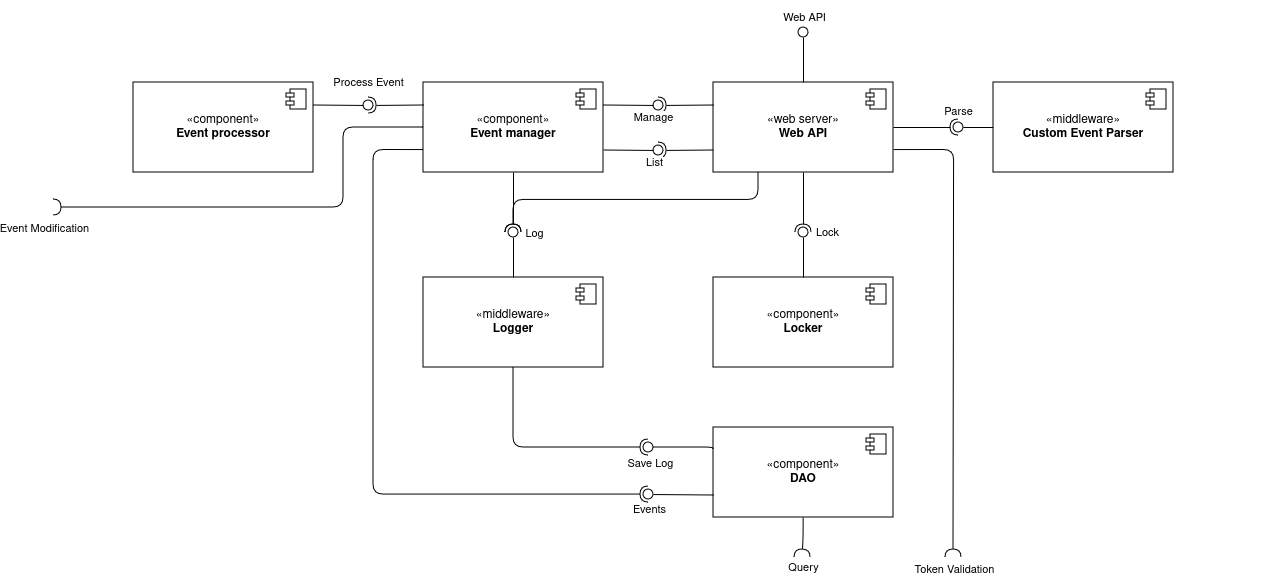
\includegraphics[width=1\textwidth]{Images/ComponentDiagram_Management.png}
    \caption{Diagramma dei componenti di \textit{Management Server}}
    \label{fig:component-diagram-management}
\end{figure}    

\subsubsection{Event processor}
\index{Event processor}

\begin{table}[htbp]
    \centering
    \renewcommand{\arraystretch}{1.3} % Imposta lo spazio verticale delle righe
    \begin{tabularx}{\textwidth}{| l | l | X |}
        \Xhline{2pt}
        \textbf{FORNITA} & \textbf{Nome} & \textbf{Descrizione} \\
        \Xhline{2pt}
         & Process event & Il componente fornisce un'interfaccia per permettere il processo degli eventi. \\
        \hline
    \end{tabularx}
    \caption{Tabella Event processor}
\end{table}


\clearpage

\subsubsection{Event Manager}
\index{Event Manager}

\begin{table}[htbp]
    \centering
    \renewcommand{\arraystretch}{1.3} % Imposta lo spazio verticale delle righe
    \begin{tabularx}{\textwidth}{| l | l | X |}
        \Xhline{2pt}
        \textbf{RICHIESTA} & \textbf{Nome} & \textbf{Descrizione} \\
        \Xhline{2pt}
         & Process event & Il componente utilizza l'interfaccia fornita dal componente \textit{Event processor} per il processo degli eventi. \\
        \hline
         & Event modification & Il componente utilizza l'interfaccia fornita dal componente \textit{Event processor} per modificare un evento. \\
        \hline
         & Log & Il componente utilizza l'interfaccia fornita dal componente \textit{Logger} per il salvataggio dello storico di tutte le operazioni effettuate. \\
        \hline
         & Events & Il componente utilizza l'interfaccia fornita dal componente \textit{DAO} per reperire tutti gli eventi a sistema. \\
        \Xhline{2pt}
        \textbf{FORNITA} & \textbf{Nome} & \textbf{Descrizione} \\
        \Xhline{2pt}
         & Manage & Il componente fornisce un'interfaccia per consentire la modifica degli eventi. \\
        \hline
         & List & Il componente fornisce un'interfaccia per permettere la visualizzazione di tutti gli eventi presenti nel sistema. \\
        \hline
    \end{tabularx}
    \caption{Tabella Event Manager}
\end{table}

\subsubsection{DAO}
\index{DAO}

\begin{table}[htbp]
    \centering
    \renewcommand{\arraystretch}{1.3} % Imposta lo spazio verticale delle righe
    \begin{tabularx}{\textwidth}{| l | l | X |}
        \Xhline{2pt}
        \textbf{RICHIESTA} & \textbf{Nome} & \textbf{Descrizione} \\
        \Xhline{2pt}
         & Query & Il componente utilizza un'interfaccia esterna per ottenere le queries da eseguire. \\
        \Xhline{2pt}
        \textbf{FORNITA} & \textbf{Nome} & \textbf{Descrizione} \\
        \Xhline{2pt}
         & Save log & Il componente fornisce un'interfaccia per permettere il salvataggio e la lettura dei log. \\
        \hline
         & Events & Il componente fornisce un'interfaccia per permettere l'accesso e la modifica di tutti gli eventi presenti nel sistema. \\
        \hline
    \end{tabularx}
    \caption{Tabella DAO}
\end{table}

\subsubsection{Custom event parser}
\index{Custom event parser}

\begin{table}[htbp]
    \centering
    \renewcommand{\arraystretch}{1.3} % Imposta lo spazio verticale delle righe
    \begin{tabularx}{\textwidth}{| l | l | X |}
        \Xhline{2pt}
        \textbf{FORNITA} & \textbf{Nome} & \textbf{Descrizione} \\
        \Xhline{2pt}
         & Parse & Il componente fornisce un'interfaccia per eseguire il parsing dei dati in formati proprietari dei vari dipartimenti. \\
        \hline
    \end{tabularx}
    \caption{Tabella Custom event parser}
\end{table}

\clearpage

\subsubsection{Web API}
\index{Web API}

\begin{table}[htbp]
    \centering
    \renewcommand{\arraystretch}{1.3} % Imposta lo spazio verticale delle righe
    \begin{tabularx}{\textwidth}{| l | l | X |}
        \Xhline{2pt}
        \textbf{RICHIESTA} & \textbf{Nome} & \textbf{Descrizione} \\
        \Xhline{2pt}
         & Lock & Il componente utilizza l'interfaccia fornita dal componente \textit{Locker} per permettere la mutua esclusione ad un evento. \\
        \hline
         & Log & Il componente utilizza l'interfaccia fornita dal componente \textit{Logger} per la consultazione dei log. \\
        \hline
         & List & Il componente utilizza l'interfaccia fornita dal componente \textit{Event manager} per reperire tutti gli eventi a sistema. \\
        \hline
         & Manage & Il componente utilizza l'interfaccia fornita dal componente \textit{Event manager} per permettere la gestione degli eventi. \\
        \hline
         & Parse & Il componente utilizza l'interfaccia fornita dal componente \textit{Custom event parser} per eseguire il parsing dei dati. \\
        \hline
         & Token validation & Il componente utilizza un'interfaccia esterna per la verifica e validazione del token di autenticazione. \\
         \textbf{FORNITA} & \textbf{Nome} & \textbf{Descrizione} \\
        \Xhline{2pt}
         & Web API & Il componente fornisce un'interfaccia per permettere l'utilizzo delle API agli applicativi coinvolti nel sistema. \\
        \hline
    \end{tabularx}
    \caption{Tabella Web API}
\end{table}

\subsubsection{Locker}
\index{Locker}

\begin{table}[htbp]
    \centering
    \renewcommand{\arraystretch}{1.3} % Imposta lo spazio verticale delle righe
    \begin{tabularx}{\textwidth}{| l | l | X |}
        \Xhline{2pt}
        \textbf{FORNITA} & \textbf{Nome} & \textbf{Descrizione} \\
        \Xhline{2pt}
         & Lock & Il componente fornisce un'interfaccia per consentire l'esclusività di modifica di un evento. \\
        \hline
    \end{tabularx}
    \caption{Tabella Locker}
\end{table}

\subsubsection{Logger}
\index{Logger}

\begin{table}[htbp]
    \centering
    \renewcommand{\arraystretch}{1.3} % Imposta lo spazio verticale delle righe
    \begin{tabularx}{\textwidth}{| l | l | X |}
        \Xhline{2pt}
        \textbf{RICHIESTA} & \textbf{Nome} & \textbf{Descrizione} \\
        \Xhline{2pt}
         & Save log & Il componente utilizza l'interfaccia fornita dal componente \textit{DAO} per salvare il log di tutti gli eventi. \\
        \Xhline{2pt}
        \textbf{FORNITA} & \textbf{Nome} & \textbf{Descrizione} \\
        \Xhline{2pt}
         & Log & Il componente fornisce un'interfaccia per fornire il log di tutti gli eventi. \\
        \hline
    \end{tabularx}
    \caption{Tabella Logger}
\end{table}

\clearpage


\section{Diagramma delle classi}
\index{Diagramma delle classi}

Nella sezione seguente verranno descritte nel dettaglio le classi che formeranno la struttura del sistema attraverso il diagramma delle classi.\\
Saranno quindi descritte, oltre alle classi, anche tutte le relazioni che intercorrono tra di esse e i ruoli dei gestori.\\

\subsection{Utente Autenticabile}
\index{Utente Autenticabile}

\begin{figure}[htbp]
	\centering
	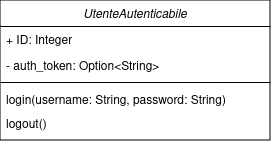
\includegraphics[width=0.25\textwidth]{Images/UtenteAutenticabile-Class.png}
	\caption{Classe Utente Autenticabile}
	\label{fig:UtenteAutenticabile}
\end{figure}

Questa classe rappresenta la figura dell'utente che utilizza l'applciazione mobile.\\
Gli utenti hanno accesso a tutte le funzionalità del sistema anche se non autenticati, quindi questa classe rappresenta tutti gli utenti che utilizzano l'applicazione e hanno le capabilities per eseguire l'accesso al sistema.\\

\textbf{Attributi:}\\

Gli attributi che caratterizzano questa classe sono:
\begin{itemize}
	\item \textbf{ID}: Attributo che rappresenta univocamente l'utente non autenticato.
	\item \textbf{auth\_token}: Attributo che rappresenta il token di autenticazione dell'utente. E' impostato ad opzionale, in quanto se l'utente non ha eseguto l'accesso questo parametro risulterà vuoto.
\end{itemize}

\textbf{Metodi:}\\

I metodi a disposizione della classe sono:
\begin{itemize}
	\item \textbf{login(username, password)}: Metodo utilizzato per effettuare il login all'interno dell'applicazione. Utilizzando questo metodo l'utente diventa un "Utente autenticato".\\Sono utilizzati metodi del gestore "Gestione utente" e del gestore "Gestione autenticazione" per effettuare il login.
	\item \textbf{logout()}: Metodo utilizzato per effettuare il logout dall'applicazione, cosi' da disconnettere l'utente dal servizio.\\
\end{itemize} 

\clearpage

\subsection{Utente}
\index{Utente}

\begin{figure}[htbp]
	\centering
	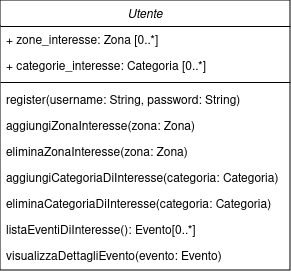
\includegraphics[width=0.25\textwidth]{Images/Utente-Class.png}
	\caption{Classe Utente}
	\label{fig:utente}
\end{figure}

La classe in questione deriva dalla classe precedente (Classe Utente, figura \ref{fig:utente}) e rappresenta tutti gli utenti che andranno ad utilizzare l'applicativo mobile.\\
Possono aver eseguito la fase di login come no, in quanto in ogni caso è garantito loro l'accesso completo alle funzionalità disponibili.\\

\textbf{Attributi:}\\
Sono a disposizione quelli della classe Utente (Figura \ref{fig:utente}), con l'aggiunta di:
\begin{itemize}
	\item \textbf{zone\_interesse}: Attributo che rappresenta le zone di interesse impostate dall'utente.
	\item \textbf{categorie\_interesse}: Attributo che rappresenta le categorie di interesse impostate dall'utente.\\
\end{itemize}

\textbf{Metodi:}\\
Anche i metodi sono gli stessi a disposizione dell'utente non autenticato, aggiungendo però il metodo:
\begin{itemize}
	\item \textbf{register(username, password)}: Metodo che permette all'utente di registrarsi per la prima volta all'interno dell'applicazione.\\Sono utilizzati metodi del gestore "Gestione utente" e del gestore "Gestione autenticazione" per effettuare la registrazione. Anche questo metodo fa diventare l'utente un "Utente autenticato".
	\item \textbf{gestioneZoneInteresse(zona)}: Metodo che permette all'utente di gestire le sue zone di interesse.
	\item \textbf{gestioneCategorieInteresse(categoria)}: Metodo che permette all'utente di gestire le sue categorie di interesse.
	\item \textbf{listaEventi()}: Metodo che permette all'utente di visualizzare la lista di tutti gli eventi presenti nel sistema.
	\item \textbf{visualizzaDettagliEvento(evento)}: Metodo che permette all'utente di visualizzare i dettagli di un singolo evento.
\end{itemize}

\clearpage

\subsection{Utente amministratore}
\index{Utente amministratore}

\begin{figure}[htbp]
	\centering
	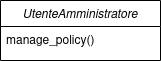
\includegraphics[width=0.25\textwidth]{Images/UtenteAmministratore-Class.png}
	\caption{Classe Utente Amministratore}
	\label{fig:utente_amministratore}
\end{figure}

La classe utente amministratore deriva dalla classe Utente Autenticabile (Figura \ref{fig:UtenteAutenticabile}) e rappresenta quell'utente con i permessi per gestire l'intero sistema.\\

Non vengono aggiunti nuovi attributi, in quanto quelli derivati dalla classe Utente Autenticabile sono sufficienti per rappresentare l'utente amministratore.\\

\textbf{Metodi:}\\
I metodi a disposizione della classe sono:

\begin{itemize}
	\item \textbf{managePolicy()}: Metodo che permette all'utente amministratore di gestire le policy del sistema.
\end{itemize}

\subsection{Utente autorizzato}
\index{Utente autorizzato}

\begin{figure}[htbp]
	\centering
	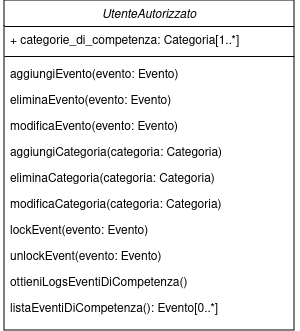
\includegraphics[width=0.3\textwidth]{Images/UtenteAutorizzato-Class.png}
	\caption{Classe Utente Autorizzato}
	\label{fig:utente_autorizzato}
\end{figure}

La classe Utente Autorizzato, anch'essa derivata da Utente Autenticabile (Figura \ref{fig:UtenteAutenticabile}) rappresenta tutti gli utenti autorizzati dal comune di Trento a pubblicare eventi e criticità a sistema.\\

\textbf{Attributi:}\\
Gli attributi che definiscono questa classe sono, oltre a quelli derivati dalla classe Utente Autenticabile, i seguenti:
\begin{itemize}
	\item \textbf{categorie\_di\_competenza}: Riporta le categorie su cui l'utente ha competenza.\\
\end{itemize}

\textbf{Metodi:}\\
I metodi a disposizione della classe sono:
\begin{itemize}
	\item \textbf{aggiungiEvento(evento)}: Metodo che permette all'utente autorizzato di creare ed aggiungere un evento al sistema.
	\item \textbf{modificaEvento(evento)}: Metodo che permette all'utente autorizzato di modificare ed aggiornare un evento precedentemente creato.
	\item \textbf{eliminaEvento(evento)}: Metodo che permette all'utente autorizzato di eliminare dal sistema un evento precedentemente creato.
	\item \textbf{aggiungiCategoria(categoria)}: Metodo che permette all'utente autorizzato di creare ed aggiungere una sottocategoria di eventi al sistema.
	\item \textbf{modificaCategoria(categoria)}: Metodo che permette all'utente autorizzato di modificare ed aggiornare una sottocategoria di eventi precedentemente creata.
	\item \textbf{eliminaCategoria(categoria)}: Metodo che permette all'utente autorizzato di eliminare dal sistema una sottocategoria di eventi precedentemente creata.
	\item \textbf{lockEvento(evento)}: Metodo che permette all'utente autorizzato di bloccare un evento per evitare che venga modificato da altri utenti (Mutua esclusione).
	\item \textbf{unlockEvento(evento)}: Metodo che permette all'utente autorizzato di sbloccare un evento precedentemente bloccato.
	\item \textbf{ottieniLogEventiDiCompetenza()}: Metodo che permette all'utente autorizzato di ottenere il log di tutti gli eventi di sua competenza.
	\item \textbf{listaEventiDiCompetenza()}: Metodo che permette all'utente autorizzato di visualizzare la lista di tutti gli eventi di sua competenza presenti nel sistema.
\end{itemize}

\clearpage

\subsection{Evento}
\index{Evento}

\begin{figure}[htbp]
	\centering
	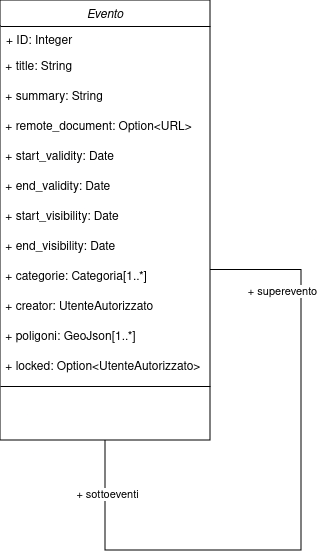
\includegraphics[width=0.25\textwidth]{Images/Evento-Class.png}
	\caption{Classe Evento}
	\label{fig:evento}
\end{figure}

La classe "Evento" rappresenta un evento o criticita' che l'utente amministratore pubblica sul sistema e che e' possibile visualizzare da applicativo mobile.

\textbf{Attributi:}\\
\begin{itemize}
	\item \textbf{ID}: Attributo che identifica univocamente l'evento pubblicato sul sistema.
	\item \textbf{title}: Attributo che rappresenta il titolo dell'evento.
	\item \textbf{summary}: Attributo che rappresenta la descrizione dell'evento.
	\item \textbf{start\_validity}: Attributo che riporta la data d'inizio validità dell'evento.
	\item \textbf{end\_validity}: Attributo che riporta la data di fine validità dell'evento.
	\item \textbf{start\_visibility}: Attributo che riporta la data d'inizio visibilità dell'evento.
	\item \textbf{end\_visibility}: Attributo che riporta la data di fine visibilità dell'evento.
	\item \textbf{categorie}: Attributo che rappresenta la categoria a cui l'evento appartiene.
	\item \textbf{sottoeventi}: Attributo che rappresenta tutti i sottoeventi che compongono l'evento stesso.
	\item \textbf{creator}: Attributo che rappresenta l'utente autorizzato che ha creato l'evento.
	\item \textbf{poligoni}: Attributo che rappresenta i poligoni che delimitano l'evento.
	\item \textbf{locked}: Attributo che rappresenta lo stato di blocco dell'evento.
\end{itemize}

Per la classe in questione non sono previsti metodi.

\clearpage 

\subsubsection{Zona}
\index{Zona}

\begin{figure}[htbp]
	\centering
	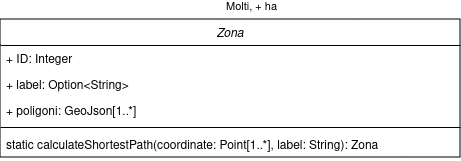
\includegraphics[width=0.5\textwidth]{Images/Zona-Class.png}
	\caption{Classe Zona d'interesse}
	\label{fig:zona}
\end{figure}

Questa classe rappresenta tutte le zone o i percorsi che risultano d'interesse per l'utente.\\

\textbf{Attributi:}\\
Gli attributi che caratterizzano questa classe sono:
\begin{itemize}
	\item \textbf{ID}: Attributo che identifica univocamente la zona d'interesse o il percorso richiesto dall'utente.
	\item \textbf{label}: Attributo che rappresenta il nome della zona d'interesse o del percorso.
	\item \textbf{poligoni}: Attributo che rappresenta i poligoni che delimitano la zona d'interesse o che disegnano il percorso.\\
\end{itemize}

\textbf{Metodi:}\\
Il metodo a disposizione della classe è:
\begin{itemize}
	\item \textbf{calculateShortestPath(coordinate)}: Metodo invocato per eseguire il calcolo del percorso più breve evitando tutte le criticita' presenti sulla mappa.
\end{itemize}

\clearpage

\subsubsection{Categoria}
\index{Categoria}

\begin{figure}[htbp]
	\centering
	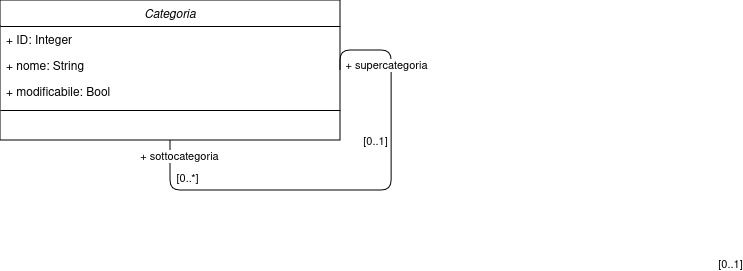
\includegraphics[width=0.5\textwidth]{Images/Categoria-Class.png}
	\caption{Classe Categoria}
	\label{fig:categoria}
\end{figure}

La classe "Categoria" rappresenta le categorie di eventi presenti sul sistema, definibili dagli utenti autorizzati dal comune di Trento.\\

\textbf{Attributi:}\\
Gli attributi che caratterizzano questa classe sono:
\begin{itemize}
	\item \textbf{ID}: Attributo che identifica univocamente la categoria di eventi.
	\item \textbf{nome}: Attributo che rappresenta il nome della categoria di eventi.
	\item \textbf{modificabile}: Attributo che rappresenta lo stato di modificabilità della categoria.\\
\end{itemize}
Per la classe in questione non sono previsti metodi.

\clearpage

\begin{figure}[htbp]
	\centering
	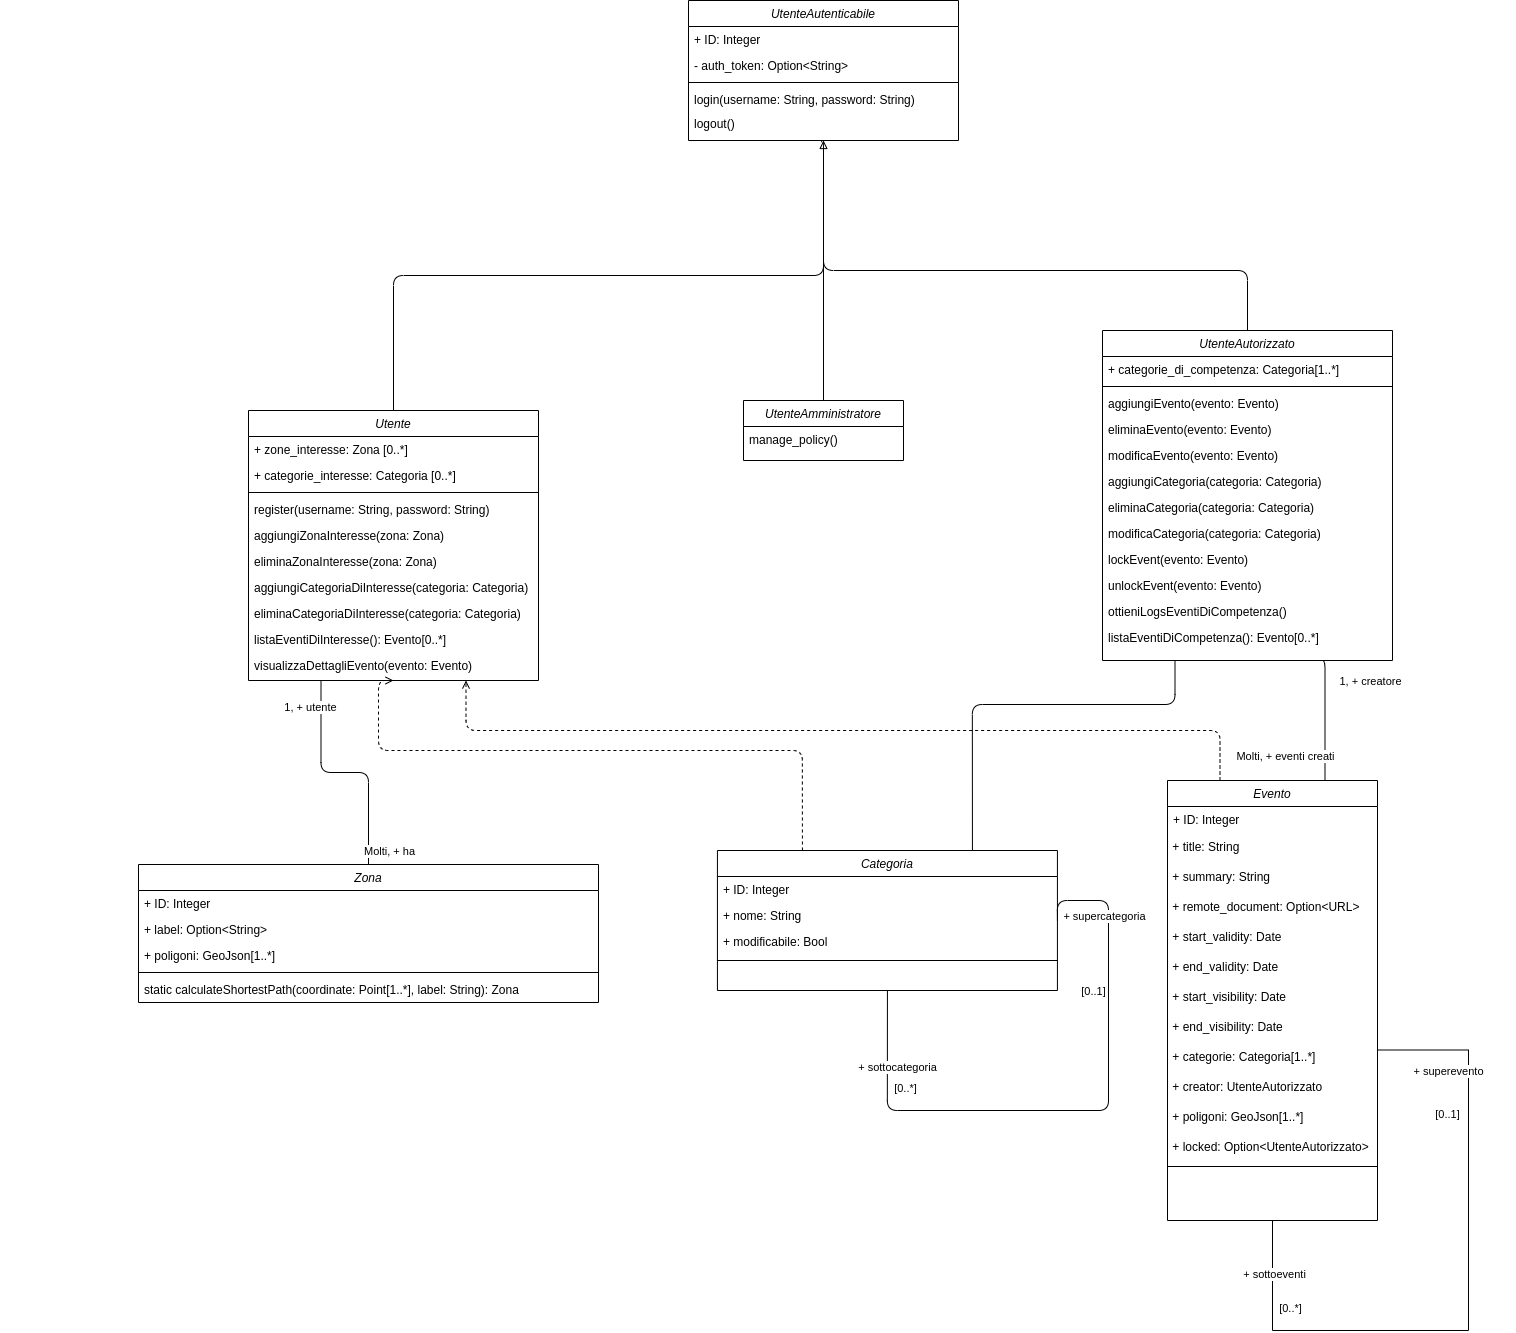
\includegraphics[width=1\textwidth]{Images/ClassDiagram.png}
	\caption{Diagramma delle classi}
	\label{fig:class-diagram}
\end{figure}


\section{Contstraints con OCL}
\index{Constraints con OCL}  

\subsection{Utente}
\index{Utente}

\begin{verbatim}
context Utente
    inv: self.zone_interesse -> forAll(z | z.utente == self)
    inv: self.percorsi -> forAll(p | p.utente == self)
    inv: self.auth_token.isEmpty() == self.is_authenticated
\end{verbatim}

\subsection{Utente autenticabile}
\index{Utente autenticabile}

\begin{verbatim}
context UtenteAutenticabile::login(_username, _password)
    pre: self.is_authenticated == false
    post: !self.auth_token.isEmpty()

context UtenteAutenticabile::deauthenticate()
    pre: self.is_authenticated == true
    post: self.auth_token.isEmpty()

context Utente::aggiungiZona(zona: ZonaDiInteresse)
    post: self.zone_interesse -> include(zona)

context Utente::aggiungiPercorso(percorso: Percorso)
    post: self.percorsi -> include(percorso)
\end{verbatim}

\subsection{Evento}
\index{Evento}

\begin{verbatim}
context Evento
    inv: self.creator.categorie_di_competenza -> includes(self.categoria)
    inv: self.creator.eventi_creati -> includes(self)
    inv: self.data_inizio <= self.data_fine
    inv: !self.info.isEmpty()
\end{verbatim}

\subsection{Categoria}
\index{Categoria}

\begin{verbatim}
# l'Admin può creare solo categorie "root" con profondità massima di 1
    inv: if instanceof(self.owner) == UtenteAmministratore:
        self.supercategoria == None || self.supecategoria->forAll(s | s.supercategoria == None)

# ogni sottoalbero di categorie deve avere una radice in un nodo "Root"
\end{verbatim}

\clearpage

\subsection{Utente Autorizzato}
\index{Utente Autorizzato}

\begin{verbatim}
context UtenteAutorizzato
    inv: self.eventi_creati -> forAll(e | e.creator == self)
    inv: self.categorie_di_competenza -> forAll()

context UtenteAutorizzato::aggiungiEvento(evento: Evento)
    post: self.eventi_creati -> include(evento)

context UtenteAutorizzato::aggiungiSottocategoria(categoria: Categoria)
    pre: !categoria.supercategoria.isEmpty()
    pre: self.categorie_di_competenza -> includes(categoria.supercategoria)
    post: self.categorie_di_competenza -> includes(categoria)
    post: categoria.owner == self

context UtenteAutorizzato::eliminaSottocategoria(categoria: Categoria)
    pre: self.categorie_di_competenza -> includes(categoria)
    pre: instanceof(categoria.owner) != UtenteAutorizzato
    post: self.categorie_di_competenza -> !includes(categoria)

context UtenteAutorizzato::modificaSottocategoria(categoria: Categoria)
    pre: self.categorie_di_competenza -> includes(categoria)
    pre: instanceof(categoria.owner) != UtenteAmministratore
    post: self.categorie_di_competenza -> includes(categoria.supercategoria)
    post: categoria.owner == categoria@pre.owner

context UtenteAutorizzato::aggiungiEvento(evento: Evento)
    post: self.categorie_di_competenza -> includes(evento.categoria)
    post: self.eventi_creati -> includes(evento)
    post: evento.creator == self

context UtenteAutorizzato::modificaEvento(evento: Evento)
    pre: evento.creator == self
    post: evento.creator == self

context UtenteAutorizzato::eliminaEvento(evento: Evento)
    pre: evento.creator == self
    post: self.eventi_creati -> !includes(evento)
\end{verbatim}

\end{document}
